\documentclass[12pt]{article}
\usepackage[top=1in,bottom=1in,left=1in,right=1in]{geometry}
\usepackage{graphicx}

\newcommand{\PstarB}{\mathcal{P}^*_B}
\newcommand{\E}{E}
\newcommand{\sigmacom}{\sigma}
\newcommand{\cmax}{1-(P^*)^{\frac1{k-1}}}
\newcommand{\PZ}{\mbox{PZ}}
\begin{document}

  \begin{figure}[tb]
    \center
    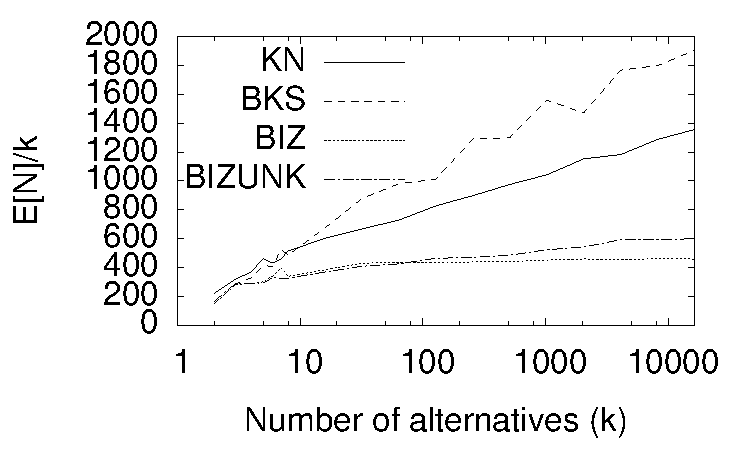
\includegraphics[width=2.9in]{QUICK-SC-Nk} 
    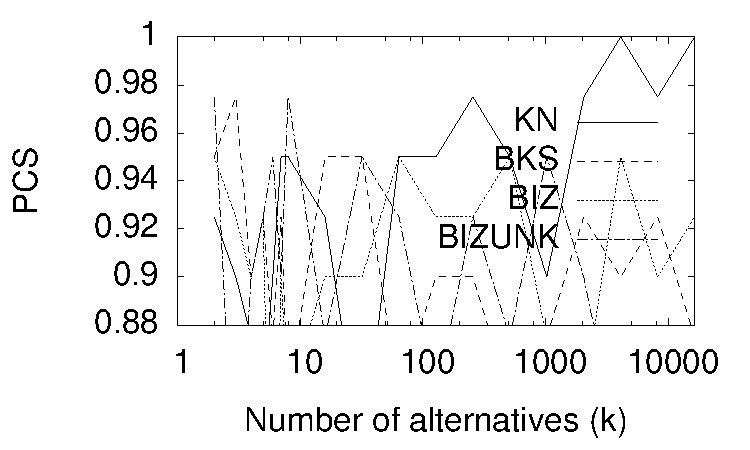
\includegraphics[width=2.9in]{QUICK-SC-PCS}
    \caption{PCS and $\E[N]/k$ as a function of the number of alternatives $k$ under the slippage configuration (SC),
    $\mu=[\delta,0,\ldots,0]$, with $P^*=0.9$, $\sigmacom=10$,
    $\delta=1$.
    BIZ uses $c=\cmax$ (eliminate aggressively).  
    BKS is the $\PstarB$ procedure.
    \label{fig:SC}}
  \end{figure}

  \begin{figure}[tb]
    \center
    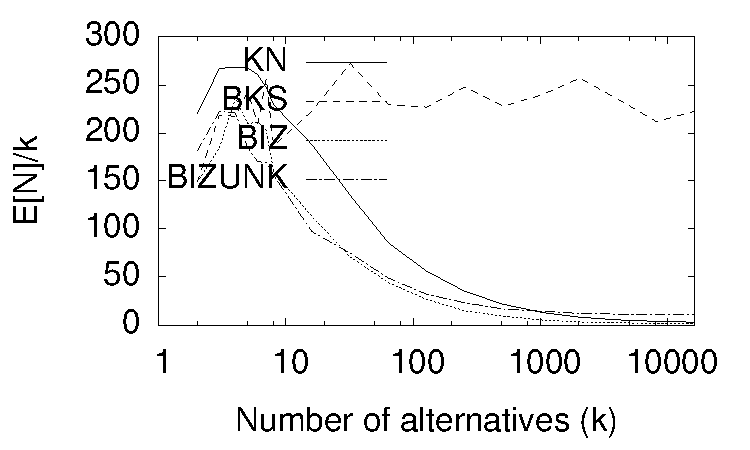
\includegraphics[width=2.9in]{QUICK-MDM-Nk} 
    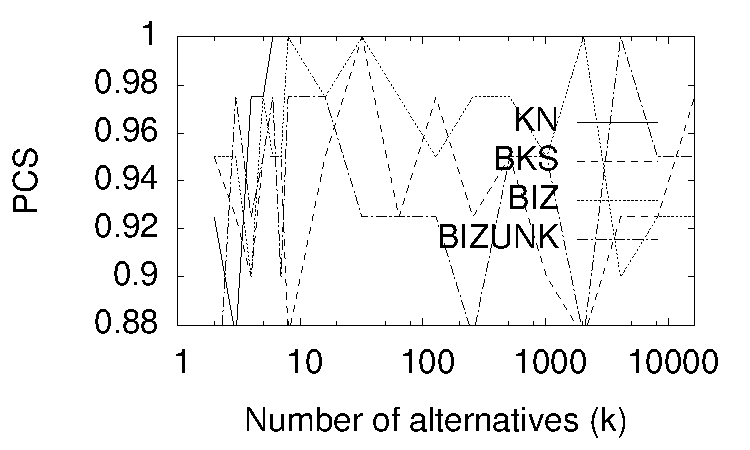
\includegraphics[width=2.9in]{QUICK-MDM-PCS}
    \caption{PCS and $\E[N]/k$ as a function of the number of alternatives $k$ under the monotone
    decreasing means (MDM) configuration, $\mu=[-\delta,-2\delta,\ldots,-k\delta]$,
    with $P^*=0.9$, $\sigmacom=10$, $\delta=1$.  
    \label{fig:MDM}}
  \end{figure}

  \begin{figure}[tb]
    \center
    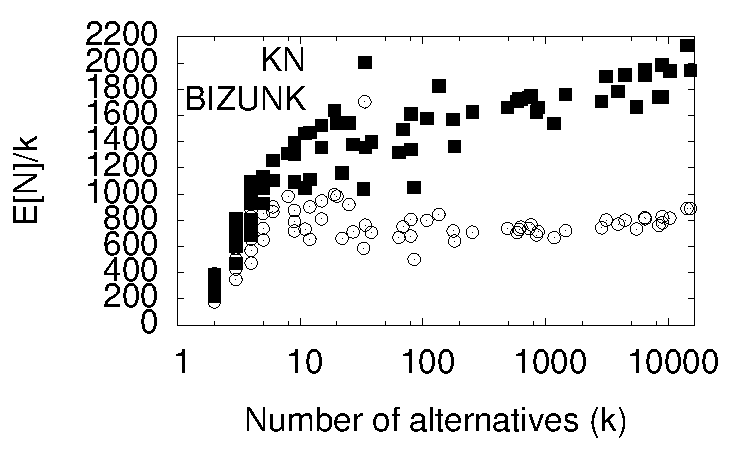
\includegraphics[width=2.9in]{QUICK-RPI-Nk}
    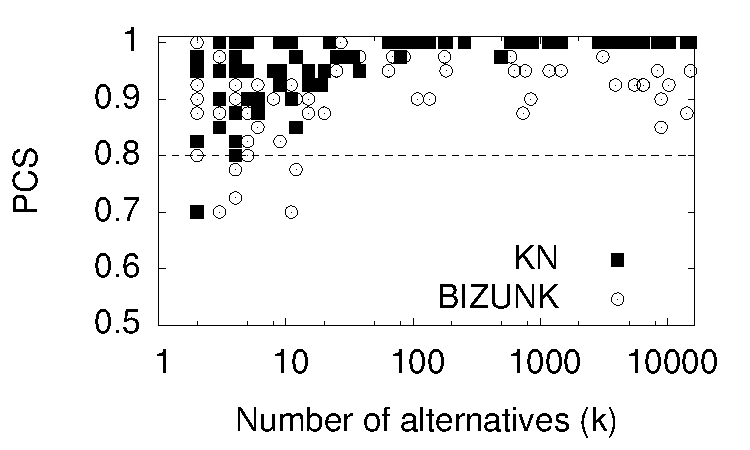
\includegraphics[width=2.9in]{QUICK-RPI-PCSk}
    \caption{Random Problem Instances:
    $P^* = 0.8$, $\sigma^2=100$, $\delta=0.5$.  Each set of sampling means $\mu$ was generated randomly from an independent normal prior and then 
    adjusted to lie in $\PZ(\delta)$.
    \label{fig:RPI}}
  \end{figure}

  \begin{figure}[tb]
    \center
    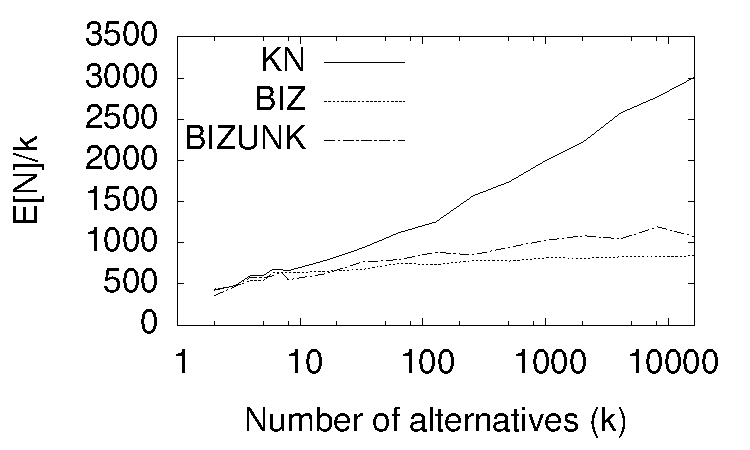
\includegraphics[width=2.9in]{QUICK-SCINC-Nk} 
    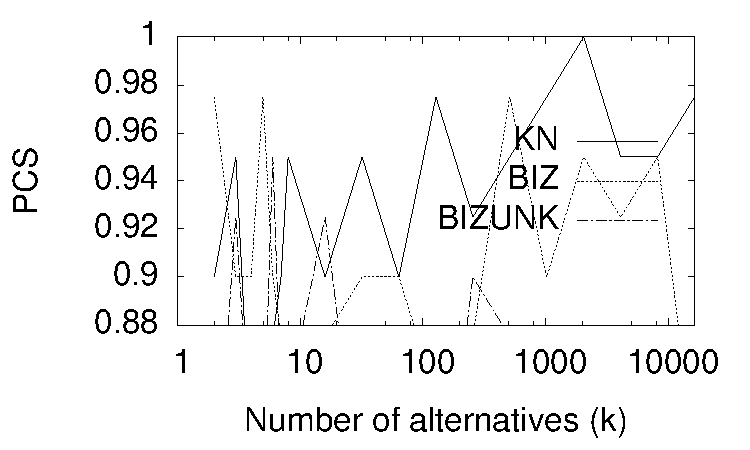
\includegraphics[width=2.9in]{QUICK-SCINC-PCS}
    \caption{SC Increasing.  
    PCS and $\E[N]/k$ as a function of the number of alternatives $k$ under the slippage configuration (SC),
    $\mu=[\delta,0,\ldots,0]$, with $P^*=0.9$, $\sigmacom=10$,
    $\delta=1$.
    BIZ uses $c=\cmax$ (eliminate aggressively).  
    \label{fig:SCINC}}
  \end{figure}
  
  \begin{figure}[tb]
    \center
    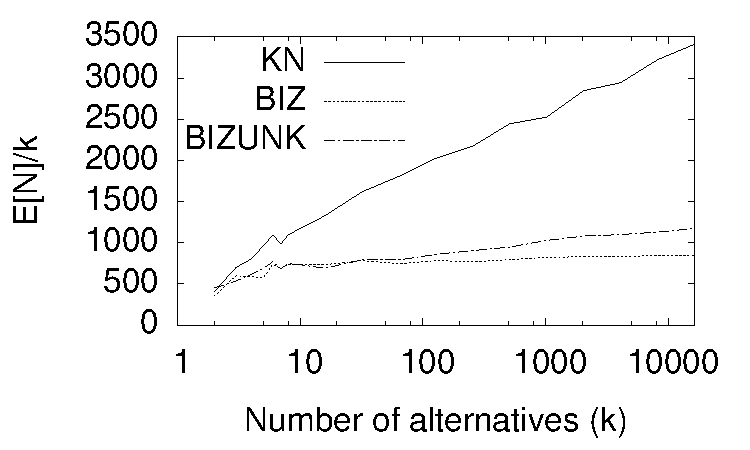
\includegraphics[width=2.9in]{QUICK-SCDEC-Nk} 
    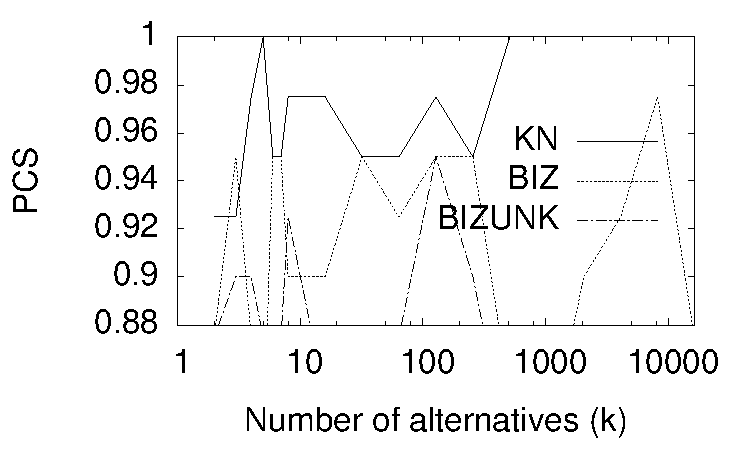
\includegraphics[width=2.9in]{QUICK-SCDEC-PCS}
    \caption{SC Decreasing.  
    PCS and $\E[N]/k$ as a function of the number of alternatives $k$ under the slippage configuration (SC),
    $\mu=[\delta,0,\ldots,0]$, with $P^*=0.9$, $\sigmacom=10$,
    $\delta=1$.
    BIZ uses $c=\cmax$ (eliminate aggressively).  
    \label{fig:SCDEC}}
  \end{figure}

  \begin{figure}[tb]
    \center
    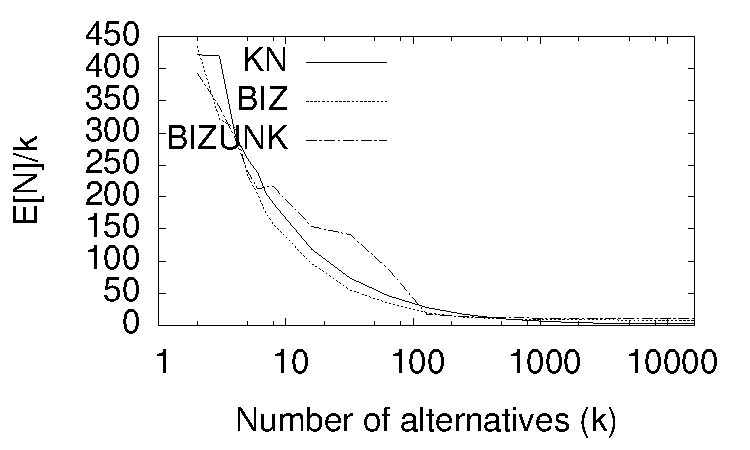
\includegraphics[width=2.9in]{QUICK-MDMINC-Nk} 
    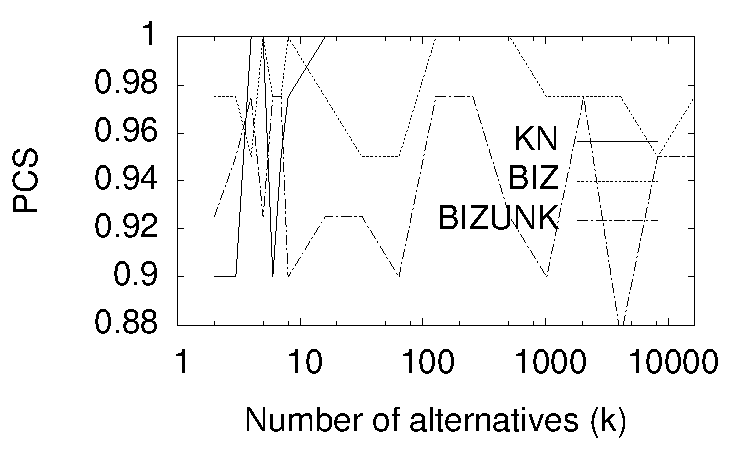
\includegraphics[width=2.9in]{QUICK-MDMINC-PCS}
    \caption{MDM Increasing.  
    PCS and $\E[N]/k$ as a function of the number of alternatives $k$ under the slippage configuration (MDM),
    $\mu=[\delta,0,\ldots,0]$, with $P^*=0.9$, $\sigmacom=10$,
    $\delta=1$.
    BIZ uses $c=\cmax$ (eliminate aggressively).  
    \label{fig:MDMINC}}
  \end{figure}
  
  \begin{figure}[tb]
    \center
    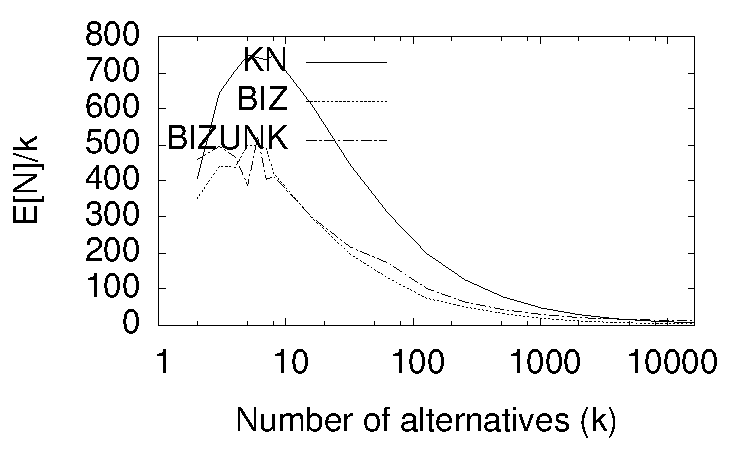
\includegraphics[width=2.9in]{QUICK-MDMDEC-Nk} 
    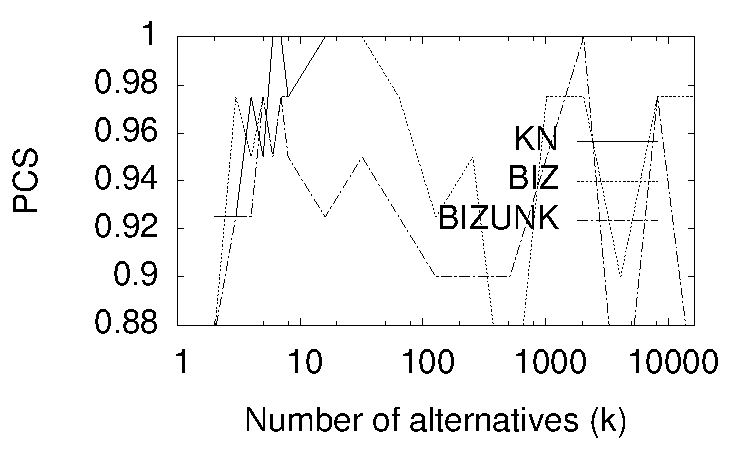
\includegraphics[width=2.9in]{QUICK-MDMDEC-PCS}
    \caption{MDM Decreasing.  
    PCS and $\E[N]/k$ as a function of the number of alternatives $k$ under the slippage configuration (MDM),
    $\mu=[\delta,0,\ldots,0]$, with $P^*=0.9$, $\sigmacom=10$,
    $\delta=1$.
    BIZ uses $c=\cmax$ (eliminate aggressively).  
    \label{fig:MDMDEC}}
  \end{figure}


  \begin{figure}[tb]
    \center
    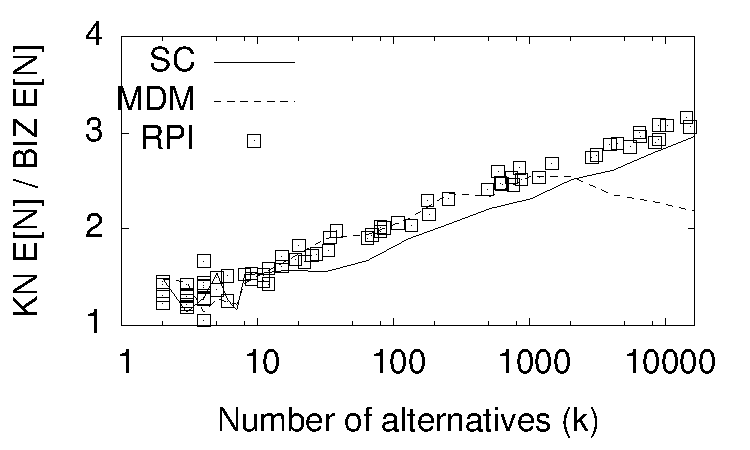
\includegraphics[width=4in]{QUICK-ImprovementFactor}
    \caption{The multiplicative improvement of BIZ over Paulson's procedure, expressed as the expected number of samples
    taken under Paulson's procedure, divided by
    the expected number of samples taken under BIZ.  This improvement is plotted for the slippage configuration (SC),
    the monotone decreasing means configurations (MDM), and random problem instances (RPI), all as a function of the number of alternatives $k$.
    % For the largest problems, BIZ requires between 10 and 15 times fewer samples than Paulson's procedure.
    \label{fig:improvement}}
  \end{figure}

 
\end{document}
